%!TEX root = ../thesis.tex
%*******************************************************************************
%*********************************** First Chapter *****************************
%*******************************************************************************

\chapter{Introduction}  %Title of the First Chapter

% \ifpdf
%     \graphicspath{{Chapter1/Figs/Raster/}{Chapter1/Figs/PDF/}{Chapter1/Figs/}}
% \else
%     \graphicspath{{Chapter1/Figs/Vector/}{Chapter1/Figs/}}
% \fi


%********************************** %First Section  **************************************
\section{Gene expression noise}

Stochastic fluctuations ("noise") of the number of 
proteins or mRNAs is common in gene expression.
Due to the randomness inherent in the kinetics of single molecules,
and environmental fluctuations, noise is generally unavoidable and
widely exists in biological processes.
Noise in gene expression is prominent since many players of the process are
typically of low copy numbers.
% The gene to be expressed usually exist in only one or a few copies
% in the genome. Transcription factors and other regulatory proteins
% can be tens to hundreds of copies in a cell, thus, contribute to the stochastic
% on-off switching of the gene. Even if the gene is actively transcribed,
% due to the short lifetime of mRNA, the number of target mRNAs in a cell at any
% given time can be low.
In a pioneering study, the authors first proposed
the concept of intrinsic noise and extrinsic noise, and demonstrated measuring
the two categories of noise by examining the correlation between two
distinguishable fluorescent reporters driven by identical promoters 
\cite{elowitz02a}.
Intrinsic noise refers to the noise from the expression mechanism per se and
extrinsic noise includes that from upstream components, e.g.
the influence of different cell states or the cell cycle, 
and from the microscopic environment.
The study shows that both intrinsic and extrinsic noise are important in
setting the cell-cell variations.
Single-molecule techniques further revealed the origin of noise in gene
expression. Studies with the sensitivity to track single protein production events
in \textit{Escherichia coli} show that proteins are expressed in "bursts"
\cite{cai06a, yu06a}.
Each protein burst is generated from a single mRNA,
the production of which is also noisy.
These studies give insight into the mechanism of gene expression noise
and provide a theoretical framework to address noise.

Noise can propagate through the gene regulatory network and cells leverage
certain network structures, or motifs, to regulate noise.
Negative autoregulation filters fluctuations and increases the robustness
of gene expression \cite{becskei00}.
Coherent feed forward loops (FFL) can filter out either activation pulses or
inactivation pulses depending on whether the output node acts as an
AND gate or OR gate.
Intuitively, since the coherent FFL consists of one direct regulation and 
one regulation in delay, the input has to persist longer than the delay to
drive the output \cite{alon06}.
However, there are theoretical limitations that prevent the noise of
both genes of a two-component system to be suppressed below the 
uncontrolled level \cite{yan19}.
In another word, the price of noise controlling for one gene
is paid by increased noise on other cellular components.
On the contrary, a positive feedback loop may amplify noise. This is 
particularly helpful when the positive feedback loop maintains bistability,
since then large enough fluctuation can flip the expression state
and drives stochastically and spontaneously switching between
activation and inactivation.
This amplification of noise can be beneficial to the bacterial 
population, as discussed in the next section.
% On a higher level, due to the interdependence of regulators and the
% products, noise can propagate through the entire pathway.
% Previous work further shows that the correlation between the noise
% of pairwise genes in yeast can be used to explore pathways 
% \cite{stewart-ornstein12}.

\subsection{Functional roles of noise}
\label{sec:functional_role_noise}

Noise in gene expression often impairs the precision of the cellular
programme. However, during the past two decades, more and more genetic
circuits are found to exploit noise to achieve gene expression dynamics
that would otherwise be impossible for deterministic systems.
One of the most important functional roles of noise is to differentiate
a clonal population (i.e. genetically identical population) in a
homogeneous environment \cite{raj08,eldar10a}.
The nature of this differentiation is stochastic, as it is implied when
an initially undistinguishable population of cells 
assume different fates.
Stochastic fate decision is important for embryo development 
in multi-cellular organisms \cite{dietrich07}.
For bacteria, noise helps to create heterogeneous phenotypes within a
population to maximize its chance of survival against 
unforeseen, fluctuating future environment.
Turning on stress response is often a heavy metabolic burden to
bacteria \cite{schweder99}.
Thus, the benefit is marginal, if any, should bacteria activate its
stress response when the stress is only transient.
It is shown both experimentally and theoretically that 
switching on the stress response in only a fraction
of the population ("bet-hedging") is the optimal strategy,
which the switching frequency should be on par with
the changing rate of the environment \cite{acar08,kussell05}.
For example, the gram-positive bacteria \textit{Bacillus subtilis}
will switch on a proportion of its population to take up environmental
DNA (i.e. to achieve competence) to increase the fitness in
adverse environments.
\textit{B. subtilis} switches to competence by expressing the 
transcription activator ComK.
Süel \textit{et al.} demonstrates that a genetic circuit consisting
ComK positive autoregulation and a slower negative feedback loop
is sufficient to drive the stochastic state-switching \cite{suel06}.
Noise is crucial in such dynamics since reducing expression noise
results in a decreased proportion of competent cells 
\cite{maamar05,suel06}.

\subsection{Noise in B. subtilis sigB circuit}

Noise plays an important role in the dynamics of \textit{B. subtilis}
$\sigma^B$, the alternative sigma factor 
(more on Section~\ref{sec:alternative_sigma_factor})
that triggers the general stress response.
Locke \textit{et al.} shows that upon energy stress, $\sigma^B$ is
activated as stochastic pulses, representing a scheme for
bacteria to hedge their bets against the fluctuating environment
\cite{locke11}.
The activation time of each pulse and the interval between pulses
are both on the level of hours.
Similar to the study of \textit{B. subtilis} ComK pathway,
the authors blocked septa formation to create elongated cell phenotypes,
which has lower intrinsic noise due to an increased cellular volume.
In elongated cells, the frequency of the pulse is reduced, which
suggests that noise drives the pulsatile expression.
In addition, the frequency of the pulses is positively regulated by
the strength of the energy stress, which represents a new regulation
paradigm (converting "amplitude modulation" to "frequency modulation").
A later work by Cabeen \textit{et al.} shows different $\sigma^B$
dynamics, i.e., upon stress response, $\sigma^B$ is activated as
a single, transient pulse, whose amplitude is modulated by 
the strength of stress \cite{cabeen17}.
However, when the upstream component (RsbR as part of the stressosome)
is altered, environmental stress triggers pulse-like dynamics.
A recent study shows that not only $\sigma^B$, but also other
alternative sigma factors (i.e. sigma factors other than
the housekeeping one, which is the primary sigma factor
activated during exponential growth), 
including $\sigma^M$, $\sigma^W$,
$\sigma^X$, $\sigma^D$, etc., adopt pulsatile expression patterns
\cite{park18a}.
In fact, these sigma factors share the same core circuit structure
as $\sigma^B$, which could account for their similar dynamics
(further explained in Section~\ref{sec:shared_circuit_structure}).
As a result, different alternative sigma factors take turns to
occupy the RNAP cores rather than the conventional 
static partitioning of the pool of RNAP cores.

% \subsection{Modelling noise}
% \subsection{Noise in bacterial stress response}

\section{Bacterial alternative sigma factor circuit}
\label{sec:alternative_sigma_factor}

% unicodes are not allowed in the content table
\subsection{The SigB circuit in \textit{B. subtilis}}

% Input and output of SigB circuit
Sigma factors are the interchangeable components of 
the RNA polymerase holoenzyme (the rest of the holoenzyme
is called the RNA polymerase core) which directs the holoenzyme
to recognize different sets of promoters \cite{osterberg11}.
%%
\textit{B. subtilis} $\sigma^B$ is the alternative sigma
factor that triggers the general stress response by 
activating a regulon of more than 150 genes, which provides
multi-purpose and preventive protection for the cell \cite{hecker07}.
%%
Since the activation of $\sigma^B$-induced regulon imposes
a significant metabolic burden \cite{schweder99},
$\sigma^B$ expression is tightly controlled by a genetic circuit
consisting of mixed transcriptional and post-translational regulations.
%%
$\sigma^B$-dependent general stress response is triggered 
by a wide range of stimuli, including environmental stress
(ethanol, salt, heat-shock or blue light, etc.) 
\cite{voelker95,gaidenko06}, energy stress (starvation or
ATP and/or GTP inhibitors, including mycophenolic acid (MPA) and
carbonyl cyanide m-chlorophenyl hydrazone (CCCP), etc.)
\cite{hecker07} and low temperature stress \cite{brigulla03}.
%%
The three categories of stress induce $\sigma^B$ expression through
independent pathways \cite{voelker95, brigulla03}.

% Regulation of SigB activation
$\sigma^B$ is regulated by a positive autoregulation and 
several positive and negative feedback loops with delay
\cite{alper96, hecker07}.
%% positive autoregulation
$\sigma^B$ activates its own expression as \textit{sigB}
gene is located in an operon induced by $\sigma^B$
\cite{kalman90}.
%% anti-sigma factor
During exponential growth, $\sigma^B$ activity is repressed by 
binding to the anti-sigma factor RsbW.
%% anti-anti-sigma factor
Upon stress, $\sigma^B$ is released through a partner-switching 
mechanism of RsbW.
The anti-anti-sigma factor RsbV
competes with $\sigma^B$ to form an alternative complex with RsbW
and thus sequesters RsbW from inhibiting $\sigma^B$ \cite{alper96}.
%% RsbW and RsbV are co-transcribed
Both RsbW and RsbV are co-transcribed with $\sigma^B$ in the
same operon driven by a $\sigma^B$-dependent promoter, 
which forms a negative and positive feedback
\cite{kalman90}.
%% phosphorylation of rsbV
On top of the regulation via protein-protein interaction is the
phosphorylation of RsbV.
RsbV can only associate with RsbW in the dephosphorylated state,
while RsbW is also a kinase of RsbV \cite{dufour94}.
Thus, RsbW inactivates RsbV and contribute to the negative feedback
loop of $\sigma^B$ expression.
%% activation through phosphatase RsbP or RsbU
When RsbV is dephosphorylated, it antagonizes the anti-sigma factor
RsbW and releases $\sigma^B$ to turn on downstream genes.
The environmental stress and energy stress uses two independent 
pathways to release the phosphatase, either RsbU (with co-factor RsbT)
or RsbP (with co-factor RsbQ), to dephosphorylate RsbV
and initiate stress response \cite{voelker95}.
%% summary
In summary, the regulatory mechanism of $\sigma^B$ features
mixed positive and negative feedback
loops involving the anti- and anti-anti-sigma factor
(Figure~\ref{fig:sigB_circuit}).
This structure of $\sigma^B$ circuit is conserved across
several gram-positive bacteria (though the anti-anti-sigma
factor is missing in some species) \cite{hecker07}.

\begin{figure}[ht]
    \centering
    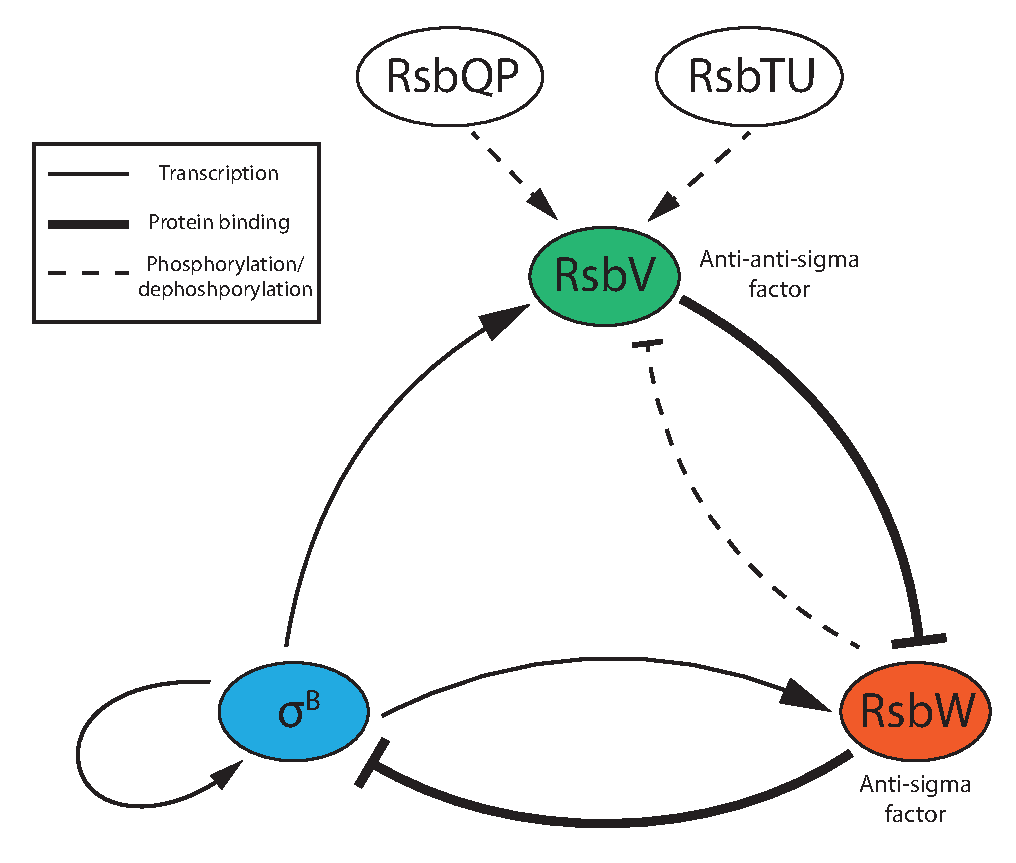
\includegraphics[width=4in]{sigB_circuit.pdf}
    \caption[
        A schematic for $\sigma^B$ gene regulation circuit.
        ]{
        \textbf{A schematic for $\sigma^B$ gene regulation circuit.}
        Type of gene/protein interaction are represented by
        different line styles.
        Pointed-end arrow denotes activation and blunt-end
        arrow denotes repression.
    }
    \label{fig:sigB_circuit}
\end{figure}

\subsection{Shared core circuit structure}
\label{sec:shared_circuit_structure}

The sigma-anti-sigma factor circuit may represent a general
regulatory mechanism for bacteria sigma factors.
Besides the aforementioned existence of $\sigma^B$ circuit
in the gram-positive relative species,
the sporulation-related sigma factors $\sigma^F$, $\sigma^E$,
and $\sigma^G$ in \textit{B. subtilis} can also be
inhibited by corresponding anti-sigma factors \cite{martinez-lumbreras18}.
Noticeably, the anti-sigma factor of $\sigma^F$, SpoIIAB,
is a kinase and can phosphorylate the anti-anti-sigma factor,
SpoIIAA. SpoIIAA can only associate with SpoIIAB when
dephosphorylated, which simulates the RsbV-RsbW-$\sigma^B$
circuit \cite{haldenwang95}.
The same structure reoccurs in \textit{E. coli}, e.g.,
the proteolysis of the general stress response sigma factor
RpoS (alias $\sigma^S$ or $\sigma^{38}$) depends on
a regulator, RssB, which serves as an anti-sigma factor
and is located in a RpoS-induced regulon.
In summary, the negative feedback loop of sigma factor conferred
by anti-sigma factor could be a general regulatory mechanism
across different bacteria species and different sigma factors
\cite{trevino-quintanilla13}.
This shared structure is reflected in the mathematical 
model for later analysis (Section~\ref{sec:low_CN}).

\subsection{Sigma factor competition}
\label{sec:intro_sigma_competition}

Besides the strict negative regulation shared among
alternative sigma factors, shifting away from the
housekeeping transcription pattern is also protected
against by the competition between sigma factors
for limited RNAP core enzymes.
%%
Sigma factor competition has been establish based on
the observation that altering housekeeping sigma factor
concentration affects the strength of alternative
sigma factor-induced stress response,
through overexpression/suppression of the housekeeping
sigma factor \cite{hicks96} or modifying the binding affinity of 
the alternative sigma factor to RNAP core \cite{zhou92a}.
%%
The alternative sigma factors (e.g. $\sigma^B$ of \textit{B. subtilis})
are at a disadvantage in the competition against the housekeeping
one since
(\textit{a}) The alternative sigma factors have weaker binding affinity
to RNAP cores than the housekeeping one, ranging from
1.5- to around 10-fold weaker \cite{maeda00,ganguly12}.
(\textit{b}) The amount of housekeeping sigma factors exceeds
significantly that of the alternative ones, even under stress
\cite{osterberg11,jishage95}.
%%
Also, considering that RNAP core and housekeeping sigma factor
roughly remains a constant level in different cell states \cite{osterberg11},
the pool of available RNAP cores for the alternative sigma factors
is capped and the competition between them can be fierce,
which is reflected a competition model that 
I developed during my research
(Section~\ref{sec:sigma_competition_model}).

\section{Biochemical ultrasensitivity}
\label{sec:biochemical_ultrasensitivity}

In the context of gene regulation, ultrasensitivity describes a sigmoidal,
switch-like increase or decrease of the expression of a gene along
increasing concentration of the regulator \cite{ferrell14a}.
%%
Namely, the dose-response curve of gene expression against regulator
concentration features a threshold, where the change of expression rate
is maximized (or "ultrasensitive" in the vicinity).
%%
The most common molecular mechanism of ultrasensitivity is binding
cooperativity, where multiple copies of the regulators associate and
together plays a role in the regulation (e.g. binds to the promoter
to initiate transcription).
%%
Conventionally, the strength of activation/repression of gene expression
is captured by the mathematical formalization of the Hill equation
\cite{hill13,alon06},
%%
where the exponent is referred to as the Hill coefficient ($n$).
When $n = 1$, the Hill equation is also referred to as the Michaelis-
Menten equation \cite{michaelis13,john12}.
%%
In equilibrium, Hill coefficient represents the number of
regulator monomers that agglomerate to form an multimer \cite{alon06}.
%%
However, often due to the lumped nature of gene expression models
(e.g. combined transcription and translation steps) and sources of
ultrasensitivity other than binding cooperativity (e.g.
multi-site phosphorylation and molecular sequestration \cite{ferrell14b}),
the Hill coefficient is an apparent parameter and is appropriate
for quantification of ultrasensitivity in the system \cite{ferrell14a}.
%%
Ultrasensitivity is crucial for a wide range of biochemical processes,
e.g., signal transduction and the maintenance of oscillation and 
bistability \cite{ferrell14c,gardner00c}.
%%
In the context of sigma factor dynamics, ultrasensitivity is needed
to explain the heterogeneity of the activation of $\sigma^V$,
where bistability is implied \cite{schwall21a}.
%%
However, there is no known binding cooperativity in most sigma
factor regulatory circuits, with one of the exceptions of \textit{B. subtilis}
$\sigma^B$ circuit, where the anti-sigma factor RsbW dimerizes and 
bind to either $\sigma^B$ or RsbV \cite{dufour94}.
The RsbW homodimer can either associate one or two monomers of
RsbV \cite{narula16}.
%%
Contradictions between the stochastic state-switching in sigma factor
dynamics and the lack of established source of ultrasensitivity
is one the main themes that I attempt to address in this thesis.
